\documentclass{beamer}

\usepackage{../../../latex_style/beamerthemeExecushares}
\usepackage{../../../latex_style/notations}

\title{Session 3: The rank}
\subtitle{Optimization and Computational Linear Algebra for Data Science}
\author{Léo Miolane}
\date{}

\setcounter{showSlideNumbers}{1}

\begin{document}
\setcounter{showProgressBar}{0}
\setcounter{showSlideNumbers}{0}

\frame{\titlepage}

\begin{frame}
	\frametitle{Contents}
	\begin{enumerate}
		\item Subspaces
		\item Linear dependency
		\item Properties of the dimension
		\item Coordinates
		\item Why do we care about all these things ? \below{Application to data science: image compression}
	\end{enumerate}
\end{frame}


\setcounter{framenumber}{0}
\setcounter{showSlideNumbers}{1}

\section{The rank}

\begin{frame}[t]{Recap of the videos}
	\vspace{-0.4cm}
	\begin{definition}
		We define the rank of a family $x_1, \dots, x_k$ of vectors of $\R^n$ as the dimension of its span:
		\vspace{-0.3cm}
		$$
		\rank(x_1, \dots, x_k) \defeq \dim (\Span(x_1, \dots, x_k)).
		\vspace{-0.3cm}
		$$
	\end{definition}
	\begin{definition}
		Let $M \in \R^{n \times m}$. Let $c_1, \dots, c_m \in \R^n$ be its columns.
		We define
		\vspace{-0.3cm}
		$$
		\rank(M) \defeq \rank(c_1, \dots, c_m) = \dim(\Im(M)).
		\vspace{-0.3cm}
		$$
	\end{definition}
	\begin{block}{Proposition}
		Let $M \in \R^{n \times m}$. Let $r_1, \dots, r_n \in \R^m$ be the rows of $M$ and $c_1, \dots, c_m \in \R^n$ be its columns.
		Then we have
		\vspace{-0.3cm}
		$$
		\rank(r_1, \dots, r_n) = \rank(c_1, \dots, c_m) = \rank(M).
		\vspace{-0.3cm}
		$$
	\end{block}
\end{frame}

\begin{frame}[t]{How do we compute the rank ?}
	\grid

	For $v_1, \dots, v_k \in \R^n$, and $\alpha \in \R \setminus \{0\}, \, \beta \in \R$ we have
	{
		\begin{align*}
			\rank(v_1, \dots, v_k)
		&=
		\rank(v_1, \dots, v_{i-1}, \, \alpha v_i \, , v_{i+1}, \dots, v_k)\\
		&=
		\rank(v_1, \dots, v_{i-1}, \, v_i + \beta v_j \, , v_{i+1}, \dots, v_k)
		\end{align*}
	}
	\vspace{2cm}
	\\
	As a consequence, the Gaussian elimination method keeps the rank of a matrix unchanged!
\end{frame}
\begin{frame}[t]{Example}
	\grid

	Let's compute the rank of \quad
	$\displaystyle
	A = 
	\begin{pmatrix}
		1  & -1 & 0 & 1 \\
		2  & 0 & 1 & -1 \\
		-1  & 5 & 2 & 0 
	\end{pmatrix}
	$

\end{frame}
\begin{frame}[t]{Example}
	\grid

\end{frame}

\section{The rank-nullity Theorem}
\begin{frame}[t]{Rank-nullity Theorem}
	\grid

	\vspace{-0.3cm}
	\begin{theorem}
		Let $L: \R^m \to \R^n$ be a linear transformation. Then
		$$
		\rank(L) + \dim(\Ker(L)) = m.
		$$
	\end{theorem}

\end{frame}

\begin{frame}[t]{Proof sketch on an example}
	\grid

	Let us solve the linear system $Ax = 0$.
	\begin{columns}
		\hspace*{-0.7cm}
		\begin{column}{0.40\textwidth}
			$$
			\left(
				\begin{array}{cccc}
					1  & -1 & 0 & 1 \\
					2  & 0 & 1 & -1 \\
					-1  & 5 & 2 & 0 
				\end{array}
				\middle|
				\begin{array}{c}
					0 \\
					0 \\
					0
				\end{array}
			\right)
			$$
			$$
			\left(
				\begin{array}{cccc}
					1  & -1 & 0 & 1 \\
					0  & 2 & 1 & -3 \\
					0  & 0 & 0 & 7 
				\end{array}
				\middle|
				\begin{array}{c}
					0 \\
					0 \\
					0
				\end{array}
			\right)
			{\color{red}
				\begin{array}{l}
					(R_1)\\
					(R_2)\\
					(R_3) -2 (R_2)
				\end{array}
			}
			$$
		\end{column}
		\begin{column}{0.55\textwidth}
			\vspace{-1.9cm}
			$$
			\left(
				\begin{array}{cccc}
					1  & -1 & 0 & 1 \\
					0  & 2 & 1 & -3 \\
					0  & 4 & 2 & 1 
				\end{array}
				\middle|
				\begin{array}{c}
					0 \\
					0 \\
					0
				\end{array}
			\right)
			{\color{red}
				\begin{array}{l}
					(R_1)\\
					(R_2) - 2 (R_1) \\
					(R_3) + (R_1)
				\end{array}
			}
			$$
		\end{column}
	\end{columns}


\end{frame}

\section{Invertible matrices}

\begin{frame}[t]{Invertible matrices}
	\grid

	\vspace{-0.3cm}

	\begin{definition}[Matrix inverse]\label{prop:matrix_inverse}
		A \textbf{square} matrix $M \in \R^{n \times n}$ is called \emph{invertible} if there exists a matrix $M^{-1} \in \R^{n \times n}$ such that 
		$$
		M M^{-1} = M^{-1} M = \Id_n.
		$$
		Such matrix $M^{-1}$ is unique and is called the \emph{inverse} of $M$.
	\end{definition}
	\textbf{Exercise}: Let $A,B \in \R^{n \times n}$. Show that if $AB = \Id_n$ then $BA = \Id_n$.

\end{frame}

\begin{frame}[t]{Invertible matrices}
	\grid

	\vspace{-0.3cm}

	\begin{block}{Theorem}
		Let $M \in \R^{n \times n}$. The following points are equivalent:
		\begin{enumerate}
			\item \label{item:th_i} $M$ is invertible.
			\item For all $y \in \R^n$, there exists a unique $x \in \R^n$ such that $Mx=y$.
			\item \label{item:th_ii} $\rank(M) = n$.
			\item \label{item:th_iii} $\Ker(M) = \{0\}$.
		\end{enumerate}
	\end{block}

\end{frame}
\begin{frame}[t]{Proof}
	\grid

	\pause
	\pause
	\pause
\end{frame}


\begin{frame}{What do we mean by << structure >> ?}
\end{frame}

\begin{frame}[t]{A toy example}
	Consider $n = 2$, that is images $v\in\R^2$ with only $2$ pixels.
\end{frame}

\begin{frame}[t]{Examples of good bases}
	\begin{itemize}
		\item \textbf{Fourier bases} (used in \texttt{.jpeg}, \texttt{.mp3})
			\begin{figure}
				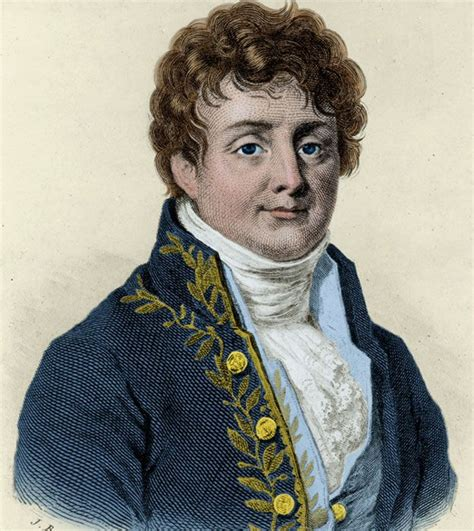
\includegraphics[height=4cm]{./fourier.jpeg}
				\hspace{1cm}
				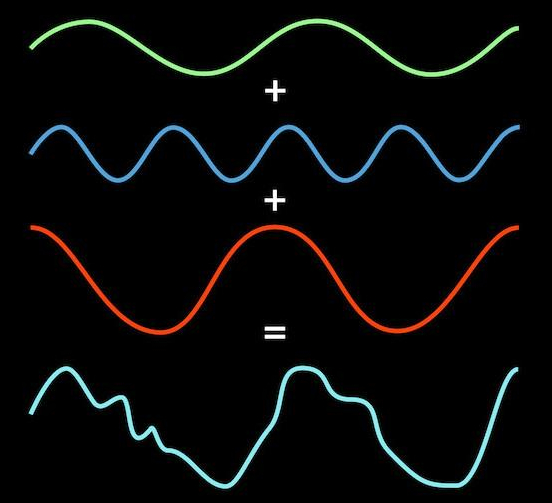
\includegraphics[height=4cm]{./fourier_dec.jpg}
			\end{figure}

		\item \texttt{JPEG2000} uses \textbf{wavelet bases}, and achieves better performance than \texttt{JPEG}.
		\item In \textbf{Homework 4}, you will use wavelets to compress/denoise images.
	\end{itemize}
\end{frame}
\appendix
\backupbegin
\begin{frame}
	\frametitle{Questions?}
\end{frame}
\backupend

\end{document}
